\documentclass[twocolumn, unnumberedsubsub]{summery_5.0} % 4.1
\title{Experimentalphysik III - Zusammenfassung}

\begin{document}
\maketitle
\tableofcontents

\section{EM-Wellen in homogener Materie}
\subsection{Maktroskopische Maxwellgleichungen}
In Materie gelten die makroskopischen Maxwellgleichungen:
\begin{empheq}{align*}
    \div \v D &= \rho\sub{frei} & \rot{ \v E} & = -\pp{\v B}t\\
    \div \v B &= 0 & \rot{\v H} &= \v j\sub{frei} + \pp{\v D}t
\end{empheq}
mit den elektrischen Feldstärke/Flussdichte $\v E/\v D$, und der magnetischen Feldstärke/Flussdichte $\v H/\v B$:
\begin{empheq}{align*}
    \v D &= \epsilon_0 \epsilon_r \v E & \v B &= \mu_0\mu_r\v H \\
    &= \epsilon_0 (\v E + \v P) & &= \mu_0 (\v H + \v M)\\
\end{empheq}

\subsection{Sammlung}
\begin{empheq}{align*}
    &\te{{\bf Allgemein:}}\\
    w &= \frac12 \epsilon_0 \hug{\v E^2 + c^2 \v B^2}\\
    \v S &= \v E \times \v H \\
    I &= \tug[]{\absv S}\\
    P\sub{st} &= \frac I c\\
    n(\lambda) &= \frac{c_0}{c(\lambda)} = \sqrt{\mu_r\epsilon_0}\\
    c &= \frac{1}{\sqrt{\mu_0\mu_r\epsilon_0\epsilon_r}} = \frac{c_0}{\sqrt{\mu_r\epsilon_r}} = \frac{c_0}n\\
    c_0 &= \frac1{\sqrt{\mu_0 \epsilon_0}}\\
    n &= \sqrt{\mu_r \epsilon_r}
\end{empheq}

\begin{empheq}{align*}
    &\te{{\bf Ebene Wellen:}}\\
    \v E &= \Re\hug{\v E_0 e^{i(\v k \v x - \omega t)}}\\
    \v B &= \frac1\omega \v k \times \v E\\
    \v S &= \frac1{\mu_0\mu_r c} \v E^2 \hat k\\
    w &= \epsilon_0 \v E^2
\end{empheq}

\begin{empheq}{align*}
    &\te{{\bf Medien:}}\\
    \v M &= \chi_m \v H = \frac{\dv m}{\dV}\\
    \v P &= \chi_e \v E = \frac{\dv p}{\dV}\\
    \epsilon_r &= 1+ \chi_e\\
    \mu_r &= 1+\chi_m\\
    n &= \frac{c_0}c= \sqrt{\epsilon_r\mu_r} = c_0 \frac k \omega = n'-i\kappa = \frac{\lambda_0}\lambda
\end{empheq}

\subsection{Mikroskopisches Modell in nichtleitendem Material}
Im klassischen Modell regt die EM-Welle die Elektronen im Material zu erzwungenen Schwingungen an. Die DGL ist:
\begin{align*}
    \ddot x + 2 \gamma \dot x + \omega_0^2 x = a(t) = -\frac{e E(t)}m = -\frac em E\sub{lok}^0 e^{i\omega t}
\end{align*} 
Für eine solche Anregung ist aus der Mechanik bekannt, dass die Amplitude der angeregten Schwingung durch 
\begin{align*}
    x(t) &= x_0 e^{i\omega t} \\
    x_0 &= -\frac{e E^0\sub{lok}}m\frac{1}{(\omega_0^2- \omega^2) + i\gamma\omega}
\end{align*}
gegeben ist. 

Die Auslenkung um \(x\) führt zu einem Dipolmoment $\v p$, und bei Dichte an Dipolmomenten $N$ zu der Polarisation $\v P$ 
\begin{align*}
    \v p &= -ex\equiv \alpha \v E\sub{lok}\\
    \v P &= N \alpha \v E\sub{lok}
\end{align*}
mit $\alpha$ als Polarisierbarkeit des Materials.

Dieser Zusammenhang kann in die makroskopische Wellengleichung mit $\v B \approx \mu_0 \v H $ 
\begin{align*}
    \Delta \v E &= \mu_0\epsilon_0 \pp[2]{\v E}t + \mu_0 \pp[2]{\v P}t
\end{align*}
eingesetzt werden, um den Brechungsindex zu berechnen:
\begin{align*}
    n^2 &= \frac{c_0^2}{c^2} = c_0^2\frac{k^2}{\omega^2} = 1+\frac{N\alpha}{\epsilon_0}
\end{align*} 
speziell für das diskutierte Modell ist der Brechungsindex somit
\begin{align*}
    \boxed{n = \sqrt{1+ \frac{e^2 N}{\epsilon_0 m (\omega_0^2 - \omega^2  + i\gamma \omega )}}}
\end{align*}
Der Brechungsindex ist also im Allgemeinen imaginär, wobei der Imaginärteil die exponentielle Absorbtion der Welle beschreibt, wie man sieht wenn man $n$ in eine Ebene Welle einsetzt:
\begin{align*}
    \v E_0 e^{i(kx - \omega t)} = \v E_0 e^{i\hug{\frac{(n'+i\kappa) \omega}c x - \omega t}}  = \v E_0 e^{-\kappa k_0 x } e^{i\hug{n' k_0 x-\omega t}}
\end{align*} 
Die Intensität geht dann, mit dem \emph{Absorbtionskoeffizienten} $A$, wie 
\begin{align*}
    I(&\v x) = c\epsilon_0 E_0^2 e^{-2\kappa \v k_0 \v x} \equiv I_0 e^{-\v A \v x}\\
    &\boxed {A = 2 \kappa k_0}
\end{align*}

Für $n\approx 1$ kann man die Näherung $n^2-1 \approx 2(n-1)$ machen, um $n'$ und $\kappa$ explizit zu erhalten:
\begin{empheq}{align*}
    n' &= 1+ \frac{N e^2}{2\epsilon_0 m} \frac{\omega_0^2 -\omega^2}{(\omega_0^2 -\omega^2)^2 + \gamma^2 \omega^2}\\
    \kappa &= \frac{N e^2}{2\epsilon_0 m} \frac{\gamma\omega}{(\omega_0^2 -\omega^2)^2 + \gamma^2 \omega^2}
\end{empheq}
Aufgrund der Dispersion sind Phasen- und Gruppengeschwindigkeit in Materie verschieden:
\begin{empheq}{align*}
\te{Phasengeschwindigkeit: }\quad c &= \frac\omega k  = \frac{c_0}{n'}\\
\te{Gruppengeschwindigkeit: }\quad c &= \pp \omega k  = \frac{c_0}{n' + \omega \pp{n'}\omega}
\end{empheq}

\subsection{Mikroskopisches Modell in leitendem Material}
In leitenden Materialien führt das E-Feld zu einem Strom $\v j = \sigma \v E$. Man erhält eine modifizierte Wellengleichung:
\begin{align*}
    \Delta \v E &= \mu_0\epsilon_0 \epsilon_r  \pp [2]{\v E}t + \mu_0 \sigma  \pp{\v E}t 
\end{align*}
das Einsetzen einer Ebenen Welle $\v E= \v E_0 e^{i(\v k\v x - \omega t)}$ 
führt dann wieder zu einem komplexen Brechungsindex
\begin{align*}
    -k^2 &= -\mu_0 \omega^2 \hug{\epsilon_0 \epsilon_r  - \frac{i \sigma}{\omega}}\\
    \implies c &= \frac\omega k = \frac{1}{\sqrt{\mu_0\hug{\epsilon_0 \epsilon_r - \frac{i\sigma}\omega}}}\\
    \implies n &= \frac{c_0}c=  \sqrt{\epsilon_r-i \frac{\sigma}{\epsilon_0\omega}}
\end{align*}
und einem Zusammenhang zwischen Brechungsindex und den Materialeigenschaften $\epsilon_r$ und $\sigma$:
\begin{align*}
    n'^2 - \kappa^2 &= \epsilon_r &
    2n'\kappa &=\frac\sigma{\epsilon_0 \omega}
\end{align*}
Man bezeichnet als \emph{Eindringtiefe} oder \emph{Skintiefe} die Strecke $\delta = 1/A $ auf der die Intensität auf $1/e$ abgefallen ist.

Für die Reaktion des Mediums auf die Welle kann die im vorherigen Teil hergeleitete Formel für den Brechungsindex verwendet werden, wenn man $\omega_0=0$ einsetzt. Mit $\omega_p$ als \emph{Plasmafrequenz}:
\begin{align*}
    \boxed{n^2 = 1- \frac{\omega_p^2}{\omega^2} \frac1{1-i\frac\gamma\omega} \te{ mit }\omega_p = \sqrt{\frac{Ne^2}{\epsilon_0 m }} }
\end{align*}
Betrachten wir nun zwei Grenzfälle:
\begin{align*}
    \omega &\ll \gamma: &  n'&=\kappa=\sqrt{\frac{\omega_p^2}{2\omega \gamma}}\\
    \omega &\gg \gamma : & n^2 &= 1- \frac{\omega_p^2}{\omega^2} 
\end{align*}
An der ersten Gleichung sieht man, dass für kleine Frequenzen Realteil gleich Imaginärteil ist, und somit starke Absorbtion auftritt.

Für große Frequenzen gibt es zwei Fälle; ist $\omega\le \omega_p$ wird der Brechungsindex rein imaginär, und die Wellen kann sich im leitendem Medium nicht ausbreiten, es kommt zur Reflektion. Für $\omega>\omega_p$ ist der Brechungsindex reell, die Absorbtion somit gering, das Material wird transparent.

\section{EM-Wellen an Grenzflächen}
\subsection{Gesetz von Snellius}
Reist ein Lichtstrahl von einem Medium $A$ mit Brechungsindex \(n_A\) in ein zweites mit Brechungindex \(n_B\), wird er gebrochen. Der Winkel kann mithilfe von Snell's Gesetz berechnet werden:
\begin{align*}
    \boxed{\frac{\sin\beta}{\sin\alpha} = \frac{n_A}{n_B}}
\end{align*}

\subsection{Totalreflexion}
Geht eine Welle von einem optisch dichten Medium in ein optisch dünnes Medium über kann es bei großen Einfallswinkel zu sog. Totalreflexion kommen, d.h. es wird die 100$\%$ der Intensität reflektiert. Ausgehend vom Gesetz von Snellius kann man den minimal Winkel für Totalreflexion herleiten, indem man fordert, dass der Ausftrittswinkel mindestens $90^\circ$ beträgt:
\begin{align*}
    \Aboxed{\sin \alpha\sub{min} &= \frac {n_B}{n_A}}
\end{align*}

\subsection{Fresnelformeln}
Es bleibt die Frage, wie sich die Intensität der einfallenden auf transmittierte und reflektierte Welle aufteilt.
Zur Herleitung des korrekten Zusammenhangs, verwendet man folgende Stetigkeitsbedingungen, welche die Welle an der Grenzfläche erfüllt:
\begin{align*}
    \v n \times (\v E_2 - \v E_1) &= 0 \qquad \v n\times(\v H_1 - \v H_1)=0\\
    \v n \cdot (\v D_2 - \v D_1) &=0\qquad \v n \cdot (\v B_2 - \v B_1)\ \ =0
\end{align*} 
Es ergeben sich für den Reflexionskoeffizient $\rho=\frac{E_r}{E_0}$ und Transmissionskoeffizienten $\tau = \frac{E_t}{E_0}$ die sog. Fresnel-Gleichungen, wobei es s- und p-Polarisation seperate Formeln gibt, und die folgenden Gleichungen nur für nicht absorbierende Medien gelten: 
\begin{boxA}
{\bf s-Polarisation:}
\begin{align*}
    \rho_s &= - \frac{\sin(\alpha-\beta)}{\sin(\alpha+\beta)}
    \qquad \tau_s = 2\frac{\cos\alpha\sin\beta}{\sin(\alpha+\beta)}
\end{align*}
{\bf p-Polarisation:}
\begin{align*}
    \rho_p &= - \frac{\tan(\alpha-\beta)}{\tan(\alpha+\beta)}
    \qquad \tau_p = \frac{2\cos\alpha\sin\beta}{\sin(\alpha+\beta)\cos(\alpha-\beta)}
\end{align*}
\end{boxA}

Auch für absorbierende Medien gelten hingegen die folgenden Gleichungen:
\begin{align*}
    \rho_s &= \frac{n_1\cos\alpha - n_2\cos\beta}{n_1\cos\alpha + n_2\cos\beta}
    \qquad \tau_s = \frac{2 n_1 \cos\alpha}{n_1\cos\alpha + n_2\cos\beta}\\
    \rho_p &= \frac{n_2\cos\alpha - n_1\cos\beta}{n_2\cos\alpha + n_1\cos\beta}
    \qquad\tau_p = \frac{2 n_2 \cos\alpha}{n_2\cos\alpha + n_1\cos\beta}
\end{align*}

Weiter gibt es für die reflektierten Wellen Phasensprünge von $\pi$ wenn $\rho$ negativ wird, und für die p-Polarisation nochmal durch die positive Definition der Schwingrichtung insgesamt ergibt sich für die Phasensprünge:
\begin{table}[H]
\centering
\setlength{\tabcolsep}{6pt}
\renewcommand{\arraystretch}{1.2}
\begin{tabular}{|cc|c|c|}
    \hline
    & & $n_2>n_1$ & $n_2<n_1$\\\hline
    p-pol: & $\alpha<\alpha_B$ & $\pi$ & $0$ \\
    & $\alpha>\alpha_B$ & 0 & $\pi$ \\\hline
    s-pol: & $\alpha<\alpha_B$ & $\pi$ & 0 \\
    & $\alpha>\alpha_B$ & $\pi$ & 0\\\hline
\end{tabular}
\end{table}
Man definiert an dieser Stelle auch noch Reflektions/Transmissionskoeffizienten für die Intensitäten:
\begin{align*}
    R &= \frac{I_R}{I_0} = \abs{\rho}^2\qquad T = \frac{I_T}{I_0} = \abs{\tau}^2
\end{align*}

\subsection{Brewsterwinkel}
Treffen p-polarisierte Wellen unter dem sog. Brewsterwinkel 
\begin{align*}
    \boxed{\tan \alpha\sub{B} = \frac{n_B}{n_A}}
\end{align*}
auf eine Grenzfläche, werden sie vollkommen transmittiert. Dies ist eine direkte Konsequenz der Fresnelformeln, und kann einfach verstanden werden, indem man sich vorstellt, dass die Wellen im Material zeitlich änderne Dipole induzieren. Herzsche Dipole emittieren keine Intensität in die Schwingrichtung ($I\propto\sin^2\alpha$), beim Brewsterwinkel handelt es sich daher einfach um den Winkel, bei dem induzierte Dipolschwingungen parallel zum reflektiertem Licht sind, also $90^\circ = \alpha+\beta$.

\subsection{Anisotrope Medien}
\begin{itemize}
    \item {\bf Optische Achse:} Die Achse, um die der Kristall die höhste Symmetrie hat. Für optisch einachsige Kristalle ist der Brechungsindex für alle senkrecht zur optischen Achse polarisierten Wellen gleich $n_o$.
    \item {\bf Ordentlicher Strahl:} Ein Strahl, welcher senkrecht zur optischen Achse polarisiert ist. Er verhält sich in einachsigen Kristallen wie in einem isotropen Material.
    \item {\bf Außerordentlicher Strahl:} Ein Strahl, welcher eine Polarisationskomponente in Richtung der optischen Achse hat (Brechungsindex $n_a$), und eine senkrecht ($n_o$). Der außerordentliche Strahl
    folgt im Allgemeinen nicht dem Brechungsgesetz und wird auch bei senkrechtem Einfall gebrochen.
\end{itemize}

\section{Polarisation}
\subsection{Definitionen}
\begin{itemize}
    \item {\bf Lineare Polarisation:}\\
    Ein Strahl, dessen \(\vec E\)-Feld in nur einer konstanten Ebene schwingt, z.B 
    $\vec E(\vec r) = \hat E e^{i(\vec k \vec r + \omega t)}$. Er kann als Superposition zweier zirkular polarisierter Strahlen dargestellt werden, 
    die konträren Drehsinn haben.
    \item {\bf Zirkulare Polarisation:}\\
    Ein Strahl, dessen \(\vec E\)-Feld im Betrag konstant ist, und um die Ausbreitungsrichtung
    kreist. Er kann als Überlagerung zweier orthogonaler, linear polarisierter
    Strahlen dargestellt werden, die zueinnander um \(90^\circ\) phasenverschoben sind.
    \begin{align*}
        \v E &= E_0 \m{\sin(kz - \omega t )\\\cos(kz - \omega t )\\0}
    \end{align*}
    \item{\bf Elliptische Polarisation:} 
    Alle anderen Polarisationen klassifiziert man als elliptisch. Jede elliptische Polarisation lässt sich darstellen als eine zirkulare Polarisation, bei der die Sinus und Cosinus Schwingungen verschiedene Amplituden haben.
    \item{\bf Polarisationsgrad:} Man definiert den Polarsationsgrad bezüglich einer bestimmen Richtungs als 
    \begin{align*}
        \Pi = \frac{I_\parallel-I_\perp}{I_\parallel+I_\perp}
    \end{align*}
\end{itemize}


\subsection{Erzeugung}
\begin{itemize}
    \item {\bf Brewstereffekt}
    \item {\bf Dichroismus:} in Effekt bei dem eine selektive Absorption einer der beiden orthogonalen Komponenten des E-Feldes stattfindet
    \item {\bf Pol-Filter:} Film aus langkettigen Kohlenwasserstoffmolekülen,
    die durch eine Streckung des Films ausgerichtet werden. Auch auf diese Weise entsteht Dichroismus, denn die Elektronen können sich entlang der ausgerichteten Molekülketten leicht bewegen und der zu den Ketten parallelen Komponente der Lichtwelle Energie entziehen.
    \item {\bf Doppelbrechende Polarisatoren} (z.B. Nicol-Prisma)
\end{itemize}

\subsection{Veränderung der Polarisation}
Wir betrachten Plättchen, die so aus einem anisotropen Kristall geschnitten wurden (parallel zur optischen Achse), das Licht welches linear in x-Richung polarisiert ist, den Brechungsindex $n_o$ erfährt, für in y-Richtung polarisiertes $n_a$. Nach Durchlaufen einer Dicke $d$ des Plättchen ist die Phasendifferenz zwischen den Komponenten dementsprechend
\begin{align*}
    \Delta \phi &= k_0 d \Delta n 
\end{align*}
\begin{itemize}
    \item {\bf $\lambda/4$-Plättchen:} Wählt man zu einer gegebenen Wellenlänge die Dicke so, dass $\Delta \phi = 90^\circ$, also $d = \frac{\lambda_0}{4\Delta n}$, dann wird in einem $45^\circ$ Winkel eintretendes linear polarisiertes Licht zu zirkular polarisiertem Licht umgewandelt. Analog wird aus zirkularer Polarisation lineare.
    \item {\bf $\lambda/2$-Plättchen:} Wählt man die Diche so, dass $\Delta \phi=180^\circ$, dann wird für linear polarisiertes Licht die Polarisationsebene entlang der optischen Achse gespiegelt, während  zirkular polarisiertes Licht die Drehrichtung wechselt.
    \item {\bf Optische aktive Flüssigkeit:} Eine optisch aktive Flüssigkeit besteht in der Regel aus chiralen Molekülen, welche verschiedene Brechungsindizes für rechts- und linksdrehendes Licht aufweist. Ein linear polarisierter Strahl dreht beim durchqueren seine Polarisationsebene.    
\end{itemize}


\section{Wellenoptik}
Eine ebene Welle wird mathematisch beschrieben durch:
\begin{align*}
    \mat E = \Im\mat E_{0} e^{i(\omega t - \mat k \cdot \mat r)}\note \mat E_0,\mat k \in\C^3\in \C^3
\end{align*}
Im Amplitudenvektor $\v E_0$ steckt die Amplitude als $\abs {E_{0,i}}$ und die 
Phasenverschiebung als $\arg \v E_{0,i}$. Damit beschreibt sie auch die Polarisation. 

\subsection{Interferenz}
Zwei oder mehr Wellenzüge überlagern sie sich nach dem Superpositionsprinzip. Die Observable der Intensität $\tug I = \epsilon_0 c \tug[]{\v E^2}$ kann bei kohärentem Licht konstruktiv oder destruktiv interferieren, es ergibt sich die folgende mittlere Intensität:
\begin{empheq}{align*}
    \tug{I} &= \tug[\big]{I_1} + \tug[\big]{I_2} + \tug[\big]{I_{12}}\\
    \tug{I_{12}} &=  2\sqrt{\tug{I_1}\tug{I_2}} \cos(\Delta \phi)
\end{empheq}

\subsection{Kohärenz}
\begin{itemize}
    \item {\bf Kohärenzzeit:}
    Zeitspanne \(\Delta t_c\) in der sich die Phasendifferenz 
    \(\Delta\phi(\v r, t) = \phi_1(\v r, t) - \phi _2(\v r, t)\) um weniger als
    \(2\pi\) ändert. 
    Man definiert hier auch die Kohärenzlänge \(\Delta l_c= c\cdot \Delta t_c\).
    \item {\bf Kohärenzlänge:}
    Wenn sich die Phasendifferenz jeder Teilwelle $i$, $\Delta \phi_i(\v r_1, \v r_2) = \psi_i(\v r_1, t) - \psi_i(\v r_2,t)$ an zwei Punkten während des eines Zeitraumes um weniger als $2\pi$ ändert dann spricht man von räumlicher Kohärenz zwischen den beiden Punkten.
    \item {\bf Kohärenzlänge realer Lichtquellen}
    Die Emission eine Wellenzuges durch ein angeregtes Atom dauert ca. 1 bis 10ns 
    (\(=\Delta t_c\)). In einem Wellenzug koexistieren verschiedene Frequenzen, die einer 
    Verteilung folgen. Man nennt \(\Delta f = \frac 1{\Delta t_c}\) die Frequenzbreite.
    Die Kohärenzlänge lasst sich in erster Näherung berechnen als 
    \(l_c = \frac{\lambda^2}{\Delta \lambda}\).
\end{itemize}


\subsection{Spalte und Gitter}
{
\subsubsection{Einzelspalt:}
Die Intensität ergibt sich als:
\begin{align*}
    I\sub{Einzelspalt}(\theta) &= I_0 \frac{\sin^2\hug{\frac{\pi}{\lambda}b\sin\theta}}{\hug{\frac\pi \lambda b \sin\theta}^2} 
\end{align*}
Für Maxima/Minima müssen die folgenden Bedingungen erfüllt sein:
\begin{align*}
    \sin\theta\sub{max} &=  \hug{n+\frac12}\frac{\lambda}{d}\\    
    \sin\theta\sub{min} &= \frac{n\lambda}{d}    
\end{align*}}\tight

\subsubsection{Doppenspalt}
    Die Intensität ergibt sich im allgemeinen Fall als die Intensitätsverteilung für einen Doppelspalt mit Spaltbreite $b=0$, welche moduliert wird durch die Verteilung eines Einzelspaltes $I =I\sub{Doppelspalt, $b=0$}\cdot I\sub{Einzelspalt}$:
    \begin{align*}
        I\sub{Doppelspalt}(\theta) & = I_0 \frac{\sin^2\hug{\frac{\pi}{\lambda}b\sin\theta}}{\hug{\frac\pi \lambda b \sin\theta}^2} \frac{\sin^2\hug{2\frac{\pi a}\lambda \sin\theta}}{\sin^2 \hug{\frac{\pi a}{\lambda} \sin\theta}}
    \end{align*}
    Für Maxima/Minima müssen die folgenden Bedingungen erfüllt sein:
    \begin{align*}
        \sin\theta\sub{max} &= \frac{n\lambda}{d}\\    
        \sin\theta\sub{min} &= \hug{n+\frac12}\frac{\lambda}{d}  
    \end{align*}\tight


\subsubsection{Gitter}
Die Intensität ergibt sich mit der Spaltanzahl $N$ als:
    \begin{align*}
        I\sub{Gitter}(\theta) &= I_0 \frac{\sin^2\hug{\frac{\pi}{\lambda}b\sin\theta}}{\hug{\frac\pi \lambda b \sin\theta}^2} \frac{\sin^2\hug{N \frac{\pi a}\lambda \sin\theta}}{\sin^2 \hug{\frac{\pi a}{\lambda} \sin\theta}}
    \end{align*}
Für Maxima/Minima müssen die folgenden Bedingungen erfüllt sein:
\begin{align*}
    \sin\theta\sub{max} &=  \frac{n\lambda}{d}\\    
    \sin\theta\sub{min} &= \hug{n+\frac12}\frac{\lambda}{d} \\   
     \sin\theta\sub{1. Nebenmin} &= \hug{n+\frac1N}\frac{\lambda}{d}\\
\end{align*}\tight


\subsubsection{Maximale Ordnung}
Es gibt eine maximale abgebildete Ordnung, denn \(1\ge\sin\alpha\). Für den Doppelspalt/Gitter würde sich ergibt sich z.B. für die maximale Ordnung der abgebildeten Maxima
\(n_{\te{max}}= \floor{\frac d\lambda}\).

\subsubsection{Überlappung von Spektren}
Die Spektren zweier benachbarter Ordnungen überlappen sich, wenn 
\(\theta_{\te{max}}(\lambda_{\te{max}}, n) > \theta_{\te{max}}(\lambda_{\te{min}}, n+1)\) gilt.
Für Doppelspalt und Gitter ergibt sich damit Überlappung für:
\begin{align*}
    n > \frac{\lambda_{\te{min}}}{\lambda_{\te{max}} - \lambda_{\te{min}}}
\end{align*}



\subsubsection{Rayleighkriterium}
Zwei Wellenlängen \(\lambda\) und \(\lambda + \Delta \lambda\) können getrennt werden, sobald das Maximum 
zu \(\lambda + \Delta \lambda\) im ersten benachbarten Minimum liegt.
Für ein Gitter ergibt sich damit: \(\frac{\lambda}{\Delta \lambda} = n N\).

\subsection{Interferenz an dünnen Schichten}
\begin{figure}[H]
    \centering
    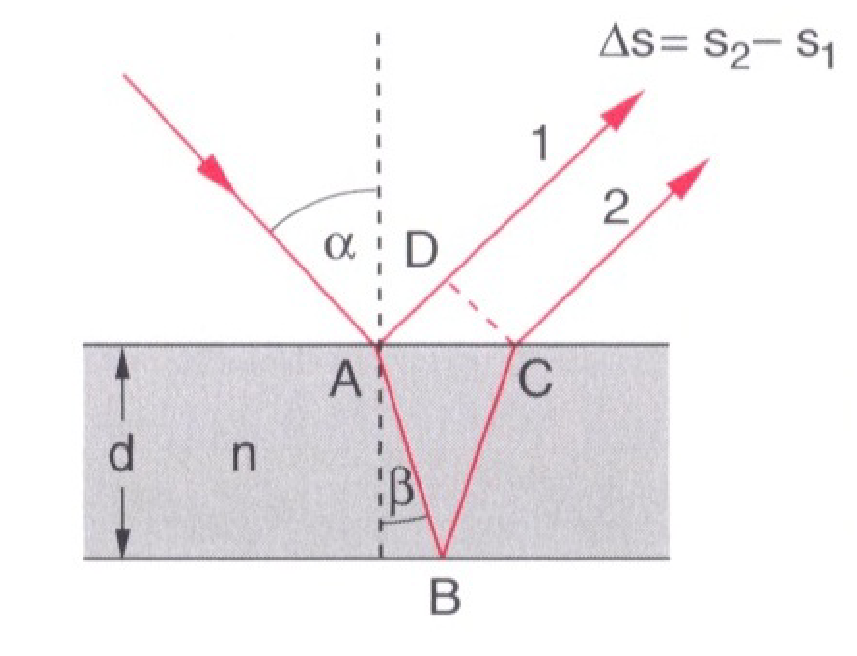
\includegraphics[width=.3\textwidth]{InteferenzAnSchichten.png}
\end{figure}
Die optische Weglängen differenz ist 
\begin{align*}
    {\Delta s = 2d \sqrt{n^2 -\sin^2\alpha}}
\end{align*}
Zusätzlich erfahren die relektierten Strahlen Phasensprünge.
Insgesamt erhält man maximale Intensität der Reflexion für
\begin{align*}
    2d\sqrt{n^2 - \sin^2\alpha} =\hug{m+\frac12} \lambda
\end{align*}

Die transmittierte Strahlung hat die gleiche optische Weglängendifferenz, erfährt aber keine Phasensprünge.
Maximale Transmission tritt auf bei:
\begin{align*}
    2d \sqrt{n^2 - \sin^2\alpha } = m \lambda
\end{align*}

\subsection{Vielstrahlinterferenz an einer dünnen Platte}
Berücksichtigt man viele interne Reflextionen und vernachlässigt die Absorbtion ergeben sich für reflektierte und transmittierte Intensität die sog. Airy-Formeln
\begin{empheq}{align*}
    I_R &= I_0 \frac{F \sin^2 \frac{\Delta\phi}{2}}{1 + F\sin^2\frac{\Delta\phi}{2}}\\
    I_T &= I_0 \frac{1}{1 + F\sin^2\frac{\Delta\phi}{2}}\\
    F &\equiv \frac{4 R}{(1-R)^2} 
\end{empheq} 

\subsection{Fabry-Perot-Interferometer}
Das Fabry-Perot-Inteferometer hat einen solchen Aufbau, dass die Airyformeln anwendbar sind. Es gibt somit maximale Transmission für
\begin{align*}
    \Delta s = 2d\sqrt{n^2-\sin^2\alpha} = m \lambda
\end{align*}
Der Transmissionskoeffizient ist als Funktion der Frequenz periodisch mit der Halbwärtsbreite
\begin{align*}
    \Aboxed{\Delta \nu = \frac c{2nd} \frac{1-R}{\pi\sqrt{R}}}
\end{align*}
Man definiert in diesem Zusammenhang auch noch die Finesse $F$, ein Maß dafür wie breit die Resonanzpeaks sind, im Verhältnis zu dem Abstand von zwei Peaks $\delta \nu= \nu_{m+1}-\nu_{m}$
\begin{align*}
    \Aboxed{F = \frac{\delta \nu}{\Delta \nu} = \frac{\pi\sqrt R}{1-R}}
\end{align*}

\subsection{Dielektrische Spiegel}
\subsection{Antireflexbeschichtung}


\subsection{Beugungsphänomene}
\subsubsection*{Frauenhofer Beugung}
Abstand des Objektes zum Schirm  gro{\ss} \(\to\) Stahlen annähernd parallel
\(\to\) Beugungsbild nur Richtungsabhängig.

\subsubsection{Fresnel Beugung}
Abstand des Objektes zum Schirm \emph{nicht} gro{\ss} \(\to\) 
Stahlen nicht parallel \(\to\) Beugungsbild Distanz und Richtungsabhängig.

\subsubsection{Fresnel-Kirchhoff'sches Beugungsintegral}
Die Amplitude und Phase auf einem Schirm \((z=0)\) sei durch \(\vec E_0(x,y)\) 
und \(\phi(x,y)\) gegeben. Dann ist die Amplitude an einem
Punkt $P=(x,y,z)^T$:
\begin{align*}
    \vec E_P(x,y,z) &= \iint\limits_{z=0} K(\beta)\frac{\vec E_0(x',y')}{r_A} 
    e^{i(\phi(x',y') - k r_A)} \dx'\dy'\\
    \te{mit } r_A &= \sqrt{(x-x')^2 + (y-y')^2 + z^2}
\end{align*}

\subsubsection{Fresnel-Linse}\tight
\begin{align*}
        &\te{Radien:}  & r_n &= 
        \sqrt{n\lambda f + \frac{n^2\lambda^2}4} \overset{f\gg n\lambda}{\approx} \sqrt{n\lambda f}
\end{align*}

\subsubsection{Lochblende}
Position der ersten Minima und Maxima hinter einer Lochblende. 
Angegeben sind die Werte für $\frac{k D}{2\pi} \sin \theta_{min}$ bzw. 
$\frac{k D}{2\pi} \sin \theta_{max}$. 
Au{\ss}erdem ist die Intensität der Nebenmaxima im Verhältnis zum zentralen
Maximum angegeben.
\begin{figure}[H]
    \centering
    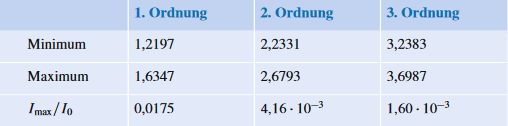
\includegraphics[width=0.5\textwidth]{2.png}
\end{figure}

\subsubsection{Rayleigh-Kriterium}
Die maximale Auflösung eines optischen Systems ist durch Beugungseffekte am 
Rand der Linse fundamental beschränkt. 
Das Rayleigh-Kriterium definiert die minimale auflösbare Winkeldistanz
als die Winkeldistanz bei der 
sich das Beugungsminimum erster Ordnung, des einen Objektes, mit dem
Beugungsmaximum erster Ordnung, des anderen Objektes, überlappen würde. 
Für eine Lochblende gilt:
\begin{align*}
    \sin\theta_{min} =  1.22 \frac{\lambda}{D}
    \ \ \implies \ \ r_{min} =  1.22 \frac{f \lambda}{D}
\end{align*}

\subsubsection{Babinet'sche Prinzip}
Das Babinet'sche Prinzip besagt, dass die Beugungsbilder zueinander komplementärer
Blenden außerhalb des Bereiches, der durch die geometrische Abbildung be-
leuchtet wird gleich ist.

\subsection{Polarisations Effekte}
\subsubsection{Definitionen}
\begin{itemize}
    \item {\bf Lineare Polarisation:}\\
    Ein Strahl, dessen \(\vec E\)-Feld in nur einer konstanten Ebene schwingt, z.B 
    $\vec E(\vec r) = \hat E e^{i(\vec k \vec r + \omega t)}$. Er kann als Superposition zweier zirkular polarisierter Strahlen dargestellt werden, 
    die konträren Drehsinn haben.
    \item {\bf Zirkulare Polarisation:}\\
    Ein Strahl, dessen \(\vec E\)-Feld im Betrag konstant ist, und um die Ausbreitungsrichtung
    kreist. Er kann als Überlagerung zweier orthogonaler, linear polarisierter
    Strahlen dargestellt werden, die zueinnander um \(90^\circ\) phasenverschoben sind.
    \item {\bf Optische Achse (Kristalloptik):}\\
    Die optische Achse ist bei einem anisotropen Kristall jene Achse, entlang derer 
    jede alle orthogonale Polarisationsrichtungen den gleichen Brechungsindex haben.
    \item {\bf Haubtschnitt:}\\
    Der Haubtschnitt ist jene Ebene, die durch die optische Achse und die Ausbreitungsrichtung 
    des Lichts aufgespannt wird.
    \item {\bf (Au{\ss}er)Ordentlicher Strahl:}\\
    Der ordentliche Teil eines Lichtstrahls ist jeder Teil dessen \(\vec E\)-Feld parallel zur optischen Achse schwingt. Die Brechungsindizes von ordentlichem und au{\ss}erordentlichem Strahl sind 
    jeweils \(n_o\) und \(n_{ao}\).
\end{itemize}

\subsubsection{Polarisationsfilter (Gesetz von Malus)}
\begin{align*}
    I' &= I \cdot \cos^2(\Delta \theta)
\end{align*}
\subsubsection{Lambda/4-Plättchen}
\begin{align*}
\Delta \phi &=\frac{2\pi}{\lambda} d \,\Delta n
\end{align*}
\subsubsection{Fresnel'sche Formeln}
Trifft ein Lichtstrahl unter einem Winkel \(\alpha\) zum Lot auf eine Grenzfläche 
zweier Medien mit Brechungszahlen $n_1$ und $n_2$, so wird er in
einen reflektierten und einen gebrochenen Strahl aufgespalten. Ihre
Amplituden sind durch die Reflexions- und Transmissionskoeffizienten 
für die Anteile an Polarisation in der Einfallsebene (Index p) und
senkrecht dazu (Index n) gegeben:
\begin{align*}
    r_n &= \frac{n_1\cos\alpha - n_2\cos\beta}{n_1\cos\alpha + n_2\cos\beta}\\
    r_p &= \frac{n_2\cos\alpha - n_1\cos\beta}{n_2\cos\alpha + n_1\cos\beta}\\
    t_n &= \frac{2 n_1 \cos\alpha}{n_1\cos\alpha + n_2\cos\beta}\\
    t_p &= \frac{2 n_2 \cos\alpha}{n_2\cos\alpha + n_1\cos\beta}
\end{align*}

\subsubsection{Anisotropie durch Spannung}
Setzt man ein Material unter Spannung (Kraftvektor \(\v F\)), kann das Material 
anisotrop werden. Der ordentliche Strahl ist orthogonal zu \(\v F\), der
außerordentliche parallel.

\subsubsection{Faraway Effekt}
Linear polarisiertes Licht wird reist durch ein Material, das von einerm starken 
B-Feld entlang der Ausbreitungsrichtung durchsetzt ist. Es wird dabei 
um einen Winkel \(\alpha = V\, L \, B, \ V=\te{Verdet-Konstante}\) gedreht. Es lässt sich erklären, wenn man das linear polarisierte Licht als 
Überlagerung zweier zirkular polarisierter Strahlen betrachtet. 
Die beiden Wellen regen Elektronen zu einer Kreisbahn an, die einen Dipolmoment erzeugt,
der je nach Richtung energetisch günstig oder ungünstig im B-Feld liegt.

\subsubsection{Kerr-Effekt}
Equivalent zum Faraway Effekt, jedoch wird hier ein E-Feld angelegt. Es bildet sich erneut
ein anisotropes Material, da das äußere E-Feld die Schwingungseigenschaften der Elektronen 
beeinflusst. Die optische Achse liegt entlang der E-Feld Richtung.
Die Erzeugung von Dipolen ist proportional zu \(E\), und die Ausrichtung der 
Dipole auch, insgesamt also \(\propto E^2\):
\begin{align*}
    \Delta n &= n_{ao} - n_o = K \lambda E^2\note K=\te{Kerr-Konstante}\\
    \Delta \phi &= 2\pi L K E^2
\end{align*}

\subsubsection{Pockels-Effekt}
Wie Kerr-Effekt, jedoch linear in \(E\). Der Effekt ist um mindestens eine 
Größenordnung stärker als der Kerr-Effekt, bei gleicher Feldstärke.
Der Effekt ist stark Richtungsabhängig.
\begin{align*}
    \Delta n &= n_{ao} - n_o = n^3 r_{\te{eff}} E \\
    r_{\te{eff}} &= \te{effektiver elektrischer Tensor}
\end{align*}

\subsubsection{Spiegel-Isomerie}
Eine Lösung mit chiralen Molekülen dreht den Winkel des einfallenden linear polarisierten
Licht. 
\begin{align*}
    \alpha &= [\alpha]^T_\lambda \cdot \beta \cdot L \\
    [\alpha]^T_\lambda &= \te{spezifischer Drehwinkekl}\\
    \beta &= \te{Konzentration}\\ 
\end{align*}

\section{Strahlenoptik}
\subsection{Fermat's Prinzip}
Die geometrische Optik lässt sich mathematisch elegant beschreiben wenn man den Lichtweg 
\(L = \int \abs{\vec r(t)}\cdot n(\vec r (t)) \dt\) definiert. Er ist der normale Weg, gewichtete 
mit dem lokalen Brechungsindex.
Das Licht nimmt immer den Weg, der den Lichtweg extremal werden lässt.
Zur Erinnerung: Es gilt \(n = \frac{c}{v}\)

Der Weg des Lichts kann daher formal mithilfe der Euler-Lagrange Gleichungen beschrieben werden als:
\begin{align*}
    \dd {}t \pp{\mathcal L}{\dotv x} = \pp{\mathcal L}{\vec x} \with \mathcal L = \abs{\vec r(t)}\cdot n(\vec r (t))
\end{align*}

\subsection{Allgemeine Definitionen}\tight
\begin{align*}
    &\te{Gegenstandsweite:} & g &\cong \te{Gegenstandsweite}\\
    &\te{Bildweite:} & b &\cong\te{Bildweite}\\
    &\te{Gegenstand:} & G &\cong\te{Gegenstand}\\
    &\te{Bild:} & B &\cong\te{Bild}\\
    &\te{Brennweite:} & f,f' &\cong\te{Brennpunkt}\\
    &\te{Brechkraft:} & D &= \frac1f\\
    &\te{Abbildungsmaßstab:} & \Gamma &= \frac BG = \frac bg\\
    &\te{Deutliche Sehweite:} & s_0 &= 25\,\mathrm{cm}\\
    &\te{Winkelvergrößerung:} & V &= \frac{\varepsilon}{\varepsilon_0}\\
    &\te{Numerische Apperatur:} & A_N &= n\sin\alpha\\
    &\te{Öffnungsverhältnis:} &F &= \frac{f}{D\sub{Öffnung}}\\
\end{align*}
Eine positive/negative Bildweite $b$ zeigt ein reelles/virtuelles Bild an.
Ein positives/negatives Bild $B$ zeigt eine aufrechtes/verkehrtes Bild an.  
Eine positive/negative Brennweite $f$ zeigt einen reellen/virtuellen Brennpunkt an. 
\begin{figure}[H]
    \centering
    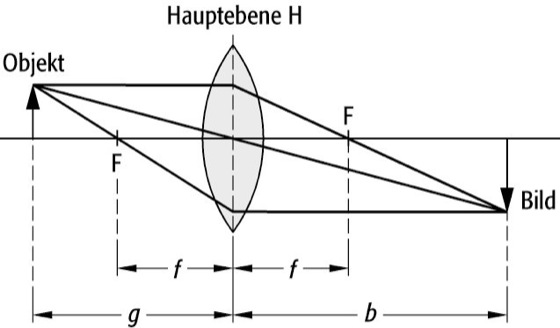
\includegraphics[width=.49\textwidth]{linse.jpg}
\end{figure}

\subsection{Listing'sche Strahlenkonstruktion}
\begin{itemize}
    \item {\bf Haubtstrahl:} Trifft auf die Mitte der Linse, die Symmetrie fordert, dass 
    der Strahl bei Linsen gerade durch geht, und bei Spiegeln mit Einfallswinkel gleich Ausfallswinkel
    reflektiert wird. 
    \item {\bf Achsenparallele:} Geht vom Gegenstand parallel zur optischen Achse. Wird in paraxialer Näherung 
    auf den Brennpunkt gebrochen (Linsen), bzw. zum Brennpunkt hin oder weg gespiegelt (Spiegel).
    \item {\bf Brennstrahl:} Analog zum Knotenpunktstrahl.
\end{itemize}

Für mehrere Linsen in einer Reihe, wird erst der (virtuelle) Bildpunkt der ersten Linse konstruiert,
anhand dessen dann der nächste Bildpunkt konstruiert wird.
Darf man sich die Gegenstandsweite auswählen, ist es meist sinnvoll diese als $g=2f$ zu wählen, da dann $g=b=2f$ und der Abstand zwischen Gegenstand und Bild minimal ist. 

\subsection{Dünne Linsen in paraxialer Näherung}

\subsubsection*{Linsengleichungen:}\tight
\begin{align*}
    \frac 1g + \frac 1b &= \frac 1f&&\te{und}&
    \frac{b}{g} &= \frac BG   
\end{align*}
Diese Gleichung gilt auch für Spiegel. Für einen konvexe Spiegel 
ist die Brennweite negativ, virtuelle Bilder haben eine negative Bildweite. \tight


\subsubsection*{Linsenmachergleichung:}\tight
\begin{align*}
    D = \frac {n_0}f = (n_L - n_0)\hug{\frac 1{r_1} + \frac 1{r_2}}
\end{align*}\ttight

\subsubsection*{Brechkraft eines optischen Systems:}\tight
\begin{align*}
    D &= D_1 + D_2 - d D_1 D_2\with d\cong \te{Distanz zwischen Linsen}
\end{align*}

\subsection{Dicke Linsen}
\subsubsection*{Linsenmachergleichung:}\tight
\begin{align*}
    D = \frac {n_0}f &= (n_L - n_0)\hug{\frac 1{r_1} + \frac 1{r_2}}
    + \frac{(n_L - n_0)^2}{n_L}\frac{d}{r_1r_2}
\end{align*}\ttight

\subsubsection*{Haubtebenen:}
\tight
\begin{align*}
    h_1 &= \frac{n_L - n_0}{n_L} \frac{f d}{r_2} & h_2 &= -\frac{n_L - n_0}{n_L} \frac{f d}{r_1}
\end{align*}\ttight

\subsubsection*{Newtonsch'sche Abbildungsgleichung}\tight
\begin{align*}
    z\cdot z' &= f_B \cdot f_G
\end{align*}\ttight

\subsubsection{Haubtebenen}
Bei dicken Linsen definiert man die sog. Haubtebenen, anhand denen die Strahlen weiterhin konstruiert werden können. Alle Größen wie $b,g$ und $f$ beziehen sich nun auf die jeweilige Haubtebene.
Die Konstruktion mit Haubteben funktioniert wie folgt:
\begin{itemize}
    \item{\bf Achsenparallele:} Ein Strahl aus dem Objektpunkt $(G)$, breitet sich parallel $(p)$ zur optischen Achse bis $H$ aus, dann parallel zur optischen Achse mit $H'$ und dann durch $f'$.
    \item{\bf Haubtstrahl:} Ein Strahl vom Objektpunkt aus auf den Schnittpunkt der Haubtebene $H$ mit der optischen Achse fällt (symmetrisch/$s$), breitet sich bis $H$ aus, dann Achsenparallel bis $H'$, und schließlich parallel zum ersten Strahl ($s$) weiter. 
    \item{\bf Brennpunktstrahl:} Ein Strahl aus dem Objektpunkt welcher durch den objektseitigen Brennpunkt $f$ geht, breitet sich bis $H$ aus, dann parallel zur optischen Achse bis $H'$ und dann weiter parallel zur optischen Achse.
\end{itemize}
Kompakt kann man die Regel für Achsenparallele/Haubtstrahl und Brennpunktstrahl kompakt zusammenfassen zu:
\begin{align*}
    G &\overset{\te{p/s/$f$}}\longrightarrow H\overset{\te{p}}\longrightarrow H' \overset{\te{$f'$/s/p}}\longrightarrow\inf
\end{align*}
\begin{figure}[H]
    \centering
    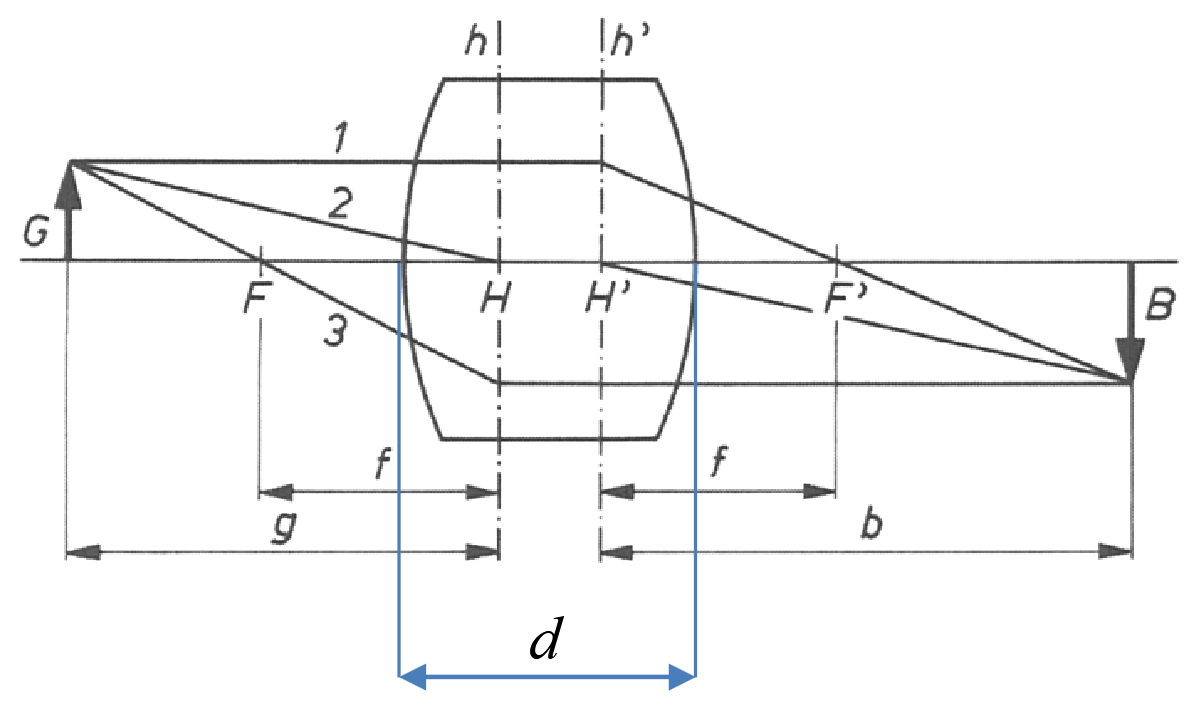
\includegraphics[width=.49\textwidth]{Haubtebenen.png}
\end{figure}


\subsection{Matrizen-Optik}
Sind vom Gegenstandspunkt aus gesehen, die vom Licht durchlaufenden Strecken \(s_1,s_2,\dots,s_n\),
so ist die korrekte Matrix gegeben durch \(M_n\cdot {\dots} \cdot M_2\cdot M_1\). Die Matrizen müssen somit 
anderrum multipliziert werden.
Ein optisches Gerät ist dann scharf eingestellt wenn \(M\cdot (0,\alpha)^T = (0,\beta)^T\).
\begin{align*}
    &\te{Zustandsvektor:} & \vec v &= \binom{x}{n\alpha}\\
    &\te{Freie Ausbreitung:} & \mat M_T &= \begin{pmatrix}
        1 & \frac{s}{n_0}\\
        0& 1
    \end{pmatrix}\\
    &\te{Brechung:} & \mat M_B &= \begin{pmatrix}
        1 & 0\\
        \frac{n_0-n_L}{R} & 1
    \end{pmatrix}\\
    &\te{Dünne Linse:} & \mat M_L &= \begin{pmatrix}
        1 & 0\\
        -D & 1
    \end{pmatrix}\\
    &\te{Dicke Linse:}
\end{align*}\tight
\begin{align*}
    \mat M_{\bar L} &= \begin{pmatrix}
        1-\frac{n_L-n_0}{n_L}\frac{d}{R_1} & \frac{d}{n_L}\\
        -D & 1+\frac{n_L-n_0}{n_L}\frac{d}{R_2}
    \end{pmatrix}
\end{align*}
 
\subsection{Bildfehler}
\begin{figure}[H]
    \centering
    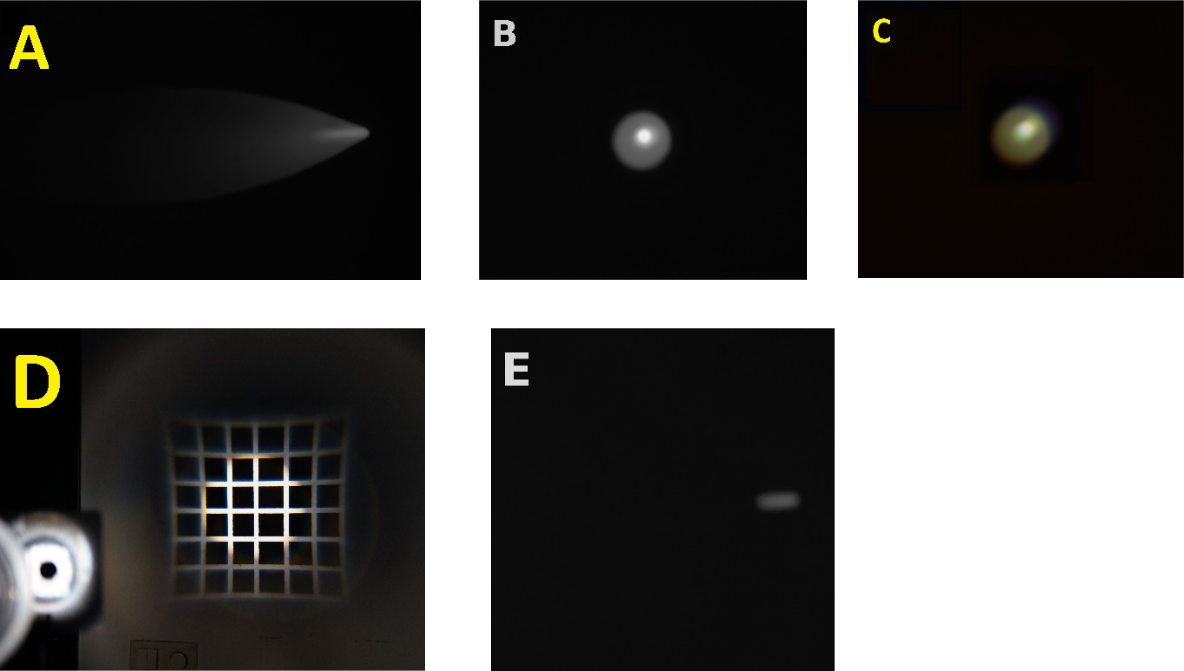
\includegraphics[width=0.4\textwidth]{3.png}
\end{figure}
\subsubsection*{A. Koma:}
Parallele Lichtstrahlen fallen in einem Winkel auf die Linse. Das Koma ist die Überlagerung zweier anderer Bildfehler,
dem Astigmatismus und der Sphärischen Abberation.\tight

\subsubsection*{B. Sphärische Abberation/Öffnungsfehler:}
Dieser Bildfehler entsteht dadurch, dass die Kugel nicht die mathematisch perfekte Form 
ist um parallele Lichtbündel auf einen Punkt zu fokossieren; dies währe ein Paraboloid.
Die Kugel ist achsenfern stärker gekrümmt als die Parabollinse, und hat daher dort eine 
stärkere Brechkraft. Der Fokuspunkt von achsenfernen Licht liegt folglich näher an der Linse. \tight

\subsubsection*{C. Chromatische Abberation:}
Die Ursache der chromatischen Abberation ist, dass die Brechkraft der Linse eine Funktion der Wellenlänge des 
Lichts ist. Folglich werden verschiedene Wellenlängen auf verschiedene Brennpunkte fokossiert. 
Ein Linsensystem das keine chromatische Abberation aufzeigt (zumindest in erster Ordung), 
also \(\pp f\lambda=0 \implies \pp{f}{n(\lambda)} =0\), nennt sich Achromat.\tight

\subsubsection*{D. Verzeichung:}
Verzeichnung ist ein Lagefehler und bedeutet, dass die Bildhöhe (Abstand eines Bildpunktes vom Bildzentrum)
auf nichtlineare Weise von der Höhe des entsprechenden Objektpunktes abhängt. Man kann auch sagen: Der Abbildungsmaßstab hängt von
der Höhe des Objektpunktes ab.h Es können sowohl kissenförmige als auch tonnenförmige Verzeichungen entstehten.\tight

\subsubsection*{E. Astigmatismus:}
Astigmatismus tritt bei "schiefen Strahlen"{} auf. die Ursache ist, dass das 
Strahlenbündel entlang der Maridional- und der Sagittalebene unterschiedlich stark gebrochen wird.

\subsection{Winkelvergrößerung}

\begin{description}
    \item[Definition:] 
    \begin{align*}
        \Aboxed{V &= \frac{\te{Winkel mit Instrument}}{\te{Winkel ohne Instrument}}=\frac{\varepsilon}{\varepsilon_0}}
    \end{align*}
    \item[Lupe:] Die Lupe ist das wohl einfachste optische Instrument. Sie besteht aus einer Sammellinse, wobei für ein aufrechtes Bild die Gegenstandsweite kleiner als die Brennweite sein muss $g\le f$. Im Fall dass $g=f$ ensteht das Bild im unendlichen, sodass es vom entspannten Auge betrachtet werden kann. In diesem Ideal ergibt sich als Winkelvergrößerung:
    \begin{align*}
        \Aboxed{V &= \frac{s_0}{f}}
    \end{align*}
    \item[Mikroskop:] Das Mikroskop besteht aus zwei Teilen: Ein {\bf Objektiv}, das ein reelles, vergrößertes Zwischenbild erzeugt (Vergrößerung $V=B/G>1$ für $f<g<2f$), und einem {\bf Okular} welches praktisch eine Lupe ist, mit der man das Zwischenbild betrachtet. Man muss darauf achten, dass die Tubuslänge auch tatsächlich lang genug ist, damit dass Zwischenbild zwischen den beiden Linsen entsteht.
    \begin{figure}[H]
        \centering
        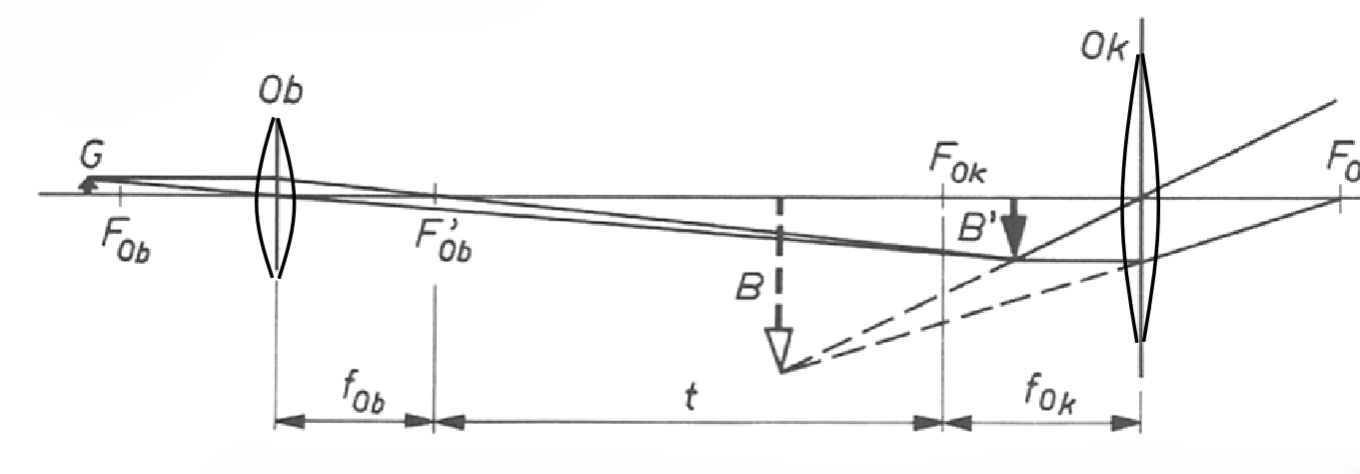
\includegraphics[width=.49\textwidth]{mikroskop.png}
        \caption{Skizze eines Mikroskop}
    \end{figure}
    Die Vergrößerung ergibt sich als:
    \begin{align*}
        \Gamma\sub{ob}&\approx \frac t{f\sub{oqb}} \with t\hat=\te{Tubuslänge} \\
        V\sub{ok} &=V\sub{Lupe} = \frac{s_0}{f\sub{ok}} \\
        \Aboxed{V\sub{Mikroskop} &= \Gamma\sub{ob} V\sub{ok} =\frac{ts_0}{f\sub{ob}f\sub{ok}} }
    \end{align*}
    \item[Teleskop:] Ein einfaches Teleskop besteht aus zwei Linsen, dessen Brennpunkte ineinander liegen. Dadurch erzeugt das Objektiv ein reelles Zwischenbild, welches man durch das Okular, wie durch eine Lupe, vergrößert betrachtet. 
    \begin{figure}[H]
        \centering
        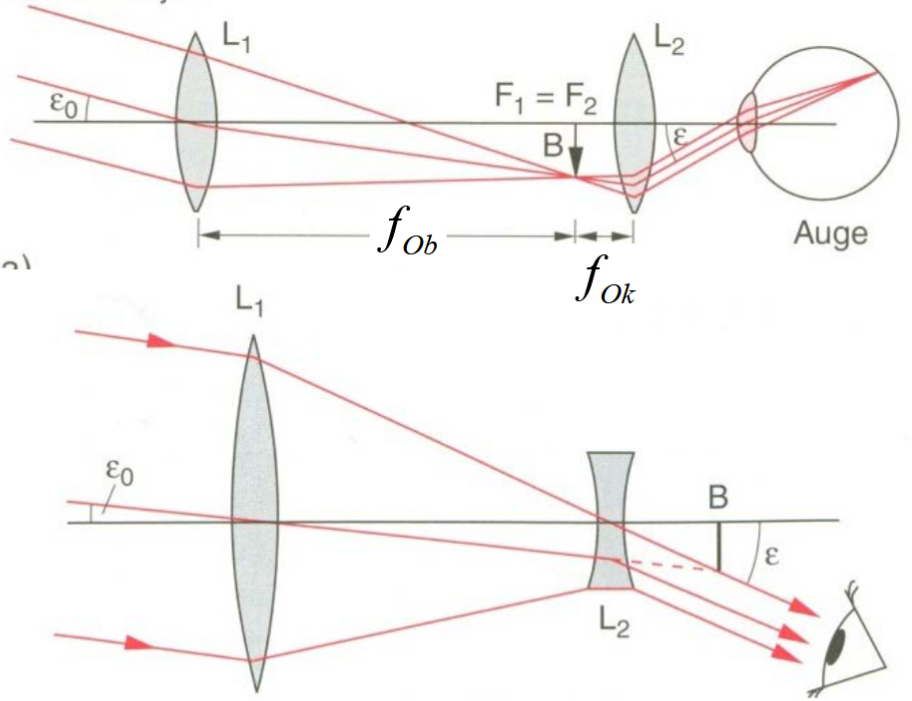
\includegraphics[width=0.49\textwidth]{fernrohr.png}
        \caption{Skizzen von 1. einem Kepler-Fernrohr, und 2. eines Galiler-Fernrohrs}
    \end{figure}
    Man kann der Skizze entnehmen, dass
    \begin{align*}
        \varepsilon &= \frac{B}{f\sub{ok}},\qquad \varepsilon_0 = \frac{B}{f\sub{ob}}
    \end{align*}
    sodass sich die Winkelvergrößerung insgesamt ergibt als:
    \begin{align*}
        \Aboxed{V\sub{Teleskop} &= \frac{f_{ob}}{f_{ok}}}
    \end{align*}
\end{description}

\subsection{Lichtstärke}
Man kann zeigen, dass die Lichtintensität in der Bildebene proportional ist zu:
\begin{align}
    \Aboxed{I \sim \frac{1}{F^2} =\hug{\frac Df}^2}
\end{align}
Wobei $F$ die sog. Blendenzahl ist.

\subsection{Schärfentiefe}
Immer wenn $g$ nicht die Linsengleichung erfüllt, entsteht in der Bildebene kein Punkt sondern ein kleines Scheibchen, das Bild ist also nicht mehr scharf. 
Solange diese Scheibchen aber kleiner sind als die Größe eines Sensorpixels $u$, ist diese Unschärfe nicht warnehmbar. Es gibt somit einen Bereich $g_\nu<g_0<g_h$ in dem das Bild scharf erscheint.
\begin{empheq}{align*}
    \Delta g_\nu &= g_0-g_\nu = \frac{u F g_0^2}{b_0 f + u F g_0} \\
    \Delta g_h &= g_h-g_0 = \frac{u F g_0^2}{b_0 f - u F g_0}
\end{empheq}
\begin{figure}[H]
    \centering
    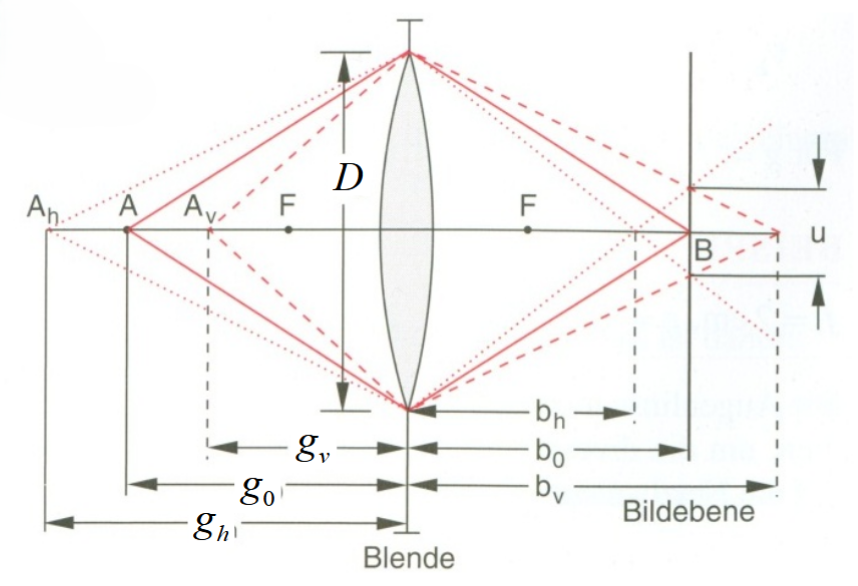
\includegraphics[width=.49\textwidth]{sch.png}
\end{figure}


\section{Optik der Atmossphäre}
\subsection{Gebogener Lichtstrahl}
\subsection{Fata Morgana}
\subsection{Regenbogen}

\section{Fotometrie}
\subsection{Allgemein}
\begin{figure}[H]
    \centering
    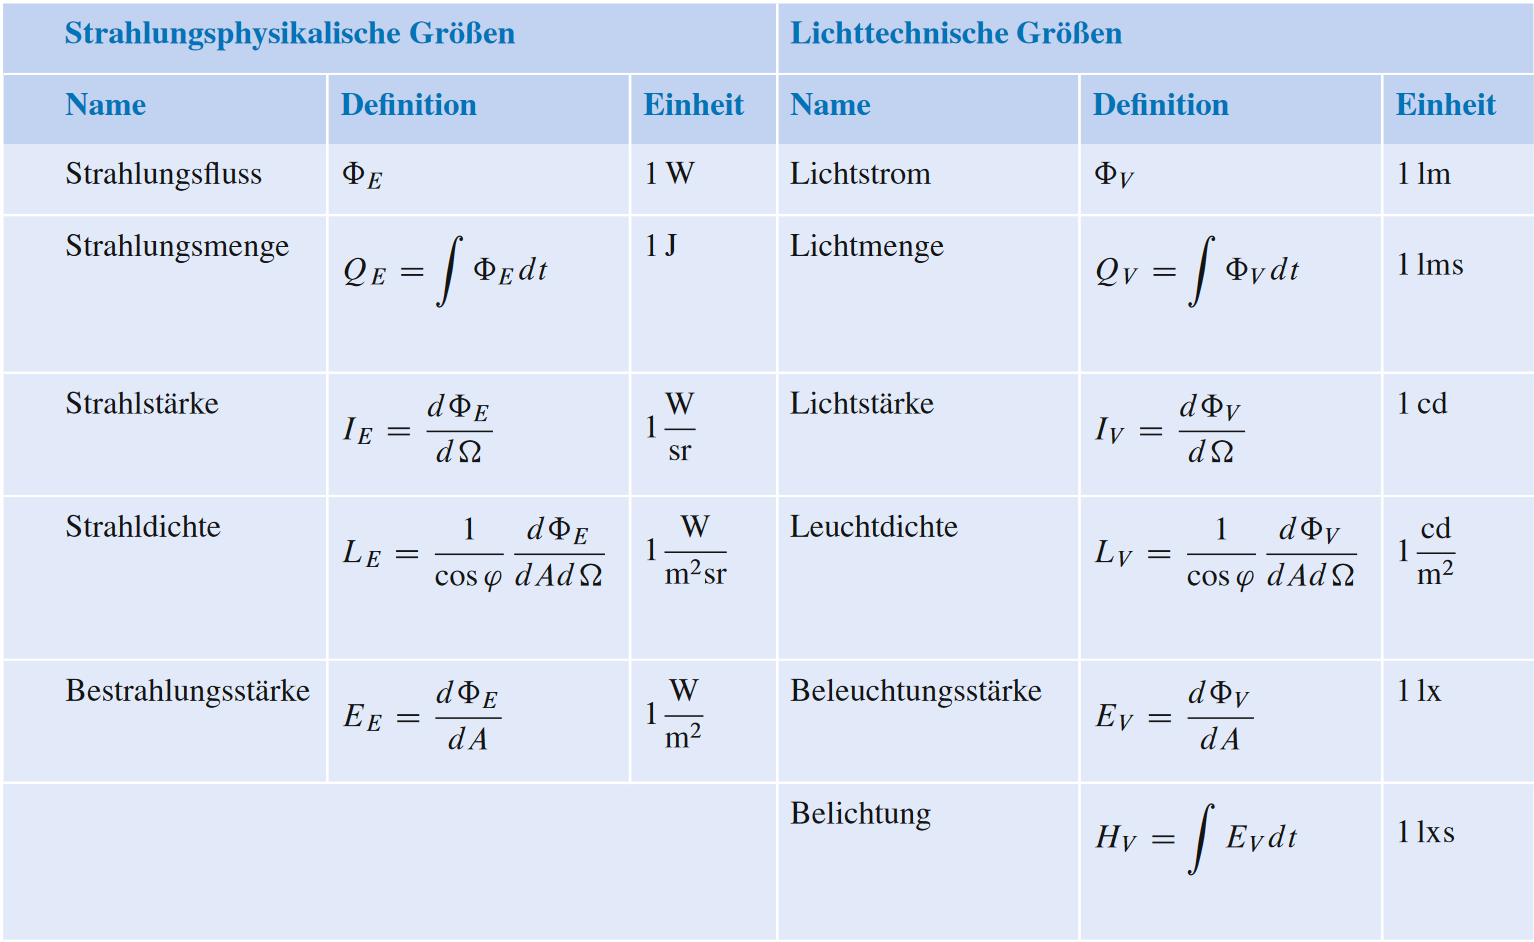
\includegraphics[width=.5\textwidth]{1.png}
\end{figure}


\subsection{Gesetze}
\subsubsection{Stefan-Boltzmann-Gesetz:}
    Gibt die Strahlungsleistung als Funktion von Fläche $A$, Temperatur $T$ und der Bolzmannkonstante $\sigma$ an: 
    \begin{align*}
        \Aboxed{\Phi_E &= \sigma \cdot A \cdot T^4}
    \end{align*}\ttight

\subsubsection{Wien'sches Verschiebungsgesetz:}
    Ist \(\lambda_{\te{max}}\) die Wellenlänge, bei der die Emission eines Schwarzerkörpers
    die maximale Intensität zeigt, so gilt:
    \begin{align*}
        \Aboxed{\lambda_{max}\cdot T = \const = 2.8978 \E{-3} \mathrm{m\, K}}
    \end{align*}\ttight

\subsubsection{Rayleigh-Jean-Gesetz:}
    Das Rayleigh-Jean-Gesetz beschreibt die Abstrahlungsleistungspektrum bei hohen Wellenlängen:
    \begin{align*}
        \Aboxed{M_E(\lambda):= \frac{\mathrm  d \Phi_E(\lambda)}{\mathrm d\lambda}=2\pi k c\frac T{\lambda^4}}
    \end{align*}\ttight

\subsubsection{Wien'sches Strahlungsgesetz:}
    Das Wien-Gesetz beschreibt die Abstrahlungsleistungspektrum bei niedrigen Wellenlängen:
    \begin{align*}
        \Aboxed{M_E(\lambda) &= \frac{c_1}{\lambda^5} \frac{1}{e^{\frac{c_2}{\lambda T}}}
        = \frac{2\pi h  c^2}{\lambda^5} \frac{1}{e^{\frac{h c}{k_B}\frac{1}{\lambda T}}}}
    \end{align*}\tight


\section{Quantenphysik}
\subsection{De-Broglie-Wellenlänge}\tight
\begin{align*}
    \v p &= \hbar \cdot \v k \rightarrow
    \lambda = \frac{h}{p}
\end{align*}

\subsection{Planksche Strahlungsformel / Schwarzkörperstrahlung}
\begin{align*}
    P(\nu) &= \frac{h \nu^3}{c^2} \frac{1}{\exp\hug{\frac{h\nu}{kT}}-1}
\end{align*}

\subsection{Compton-Effekt}
\begin{align*}
    \Delta \lambda &= \frac{h}{m_0c} (1-\cos\theta)  = \lambda_c (1-\cos\theta)
\end{align*}


\subsection{Wellenfunktion}
In der Quantenphysik dreht sich alles um die Wellenfunktion \(\psi/\Psi\), denn sie trägt alle existierenden Informationen 
über ein System gleichzeitig in sich.  
Beobachtbare Größen werden durch lineare, hermitische Operatoren beschrieben, welche auf die Wellenfunktion
wirken können.
Die Eigenvektoren eines solchen  \(\hat A \ket {A_n} = A_n\ket{A_n} \) formen eine 
vollständige, orthonormale Basis. Hat man sich eine passende Basis ausgesucht, 
kann die Wellenfunktion dieser entwickelt werden als 
\(\ket \psi = \sum_n \ket{E_n} \braket{E_n}\psi \).
Die Koeffizienten vor jedem Basisvektor, haben nach der Born-Regel eine wichtige physikalische Bedeutung:
Ihr Norm-Quadrat entspricht der Wahrscheinlichkeit, dass bei einer Messung der dem Basisvektor 
zugehörige Eigenwert gemessen wird.

\subsubsection{Schrödinger Gleichung}
Die Schrödinger Gleichung definiert dem Hamiltonoperator in Orts-Koordinaten, und kann daher verwendet werden,
um die Wellenfunktion eines Systems zu finden.

Zeitunabhängig:
\begin{align*}
        \hat H\ket \Psi&= 
        -\frac{\hbar ^2}{2m} \Delta \ket\psi + V \ket\psi
        =E\ket\psi
\end{align*}
mit \begin{align*}
    \ket{\Psi(t)} = \sum_{n} A_n e^{ {-iE_n t}/\hbar} \ket{\psi_{E_n}}
\end{align*}

Zeitabhängig:
\begin{align*}
    \hat H\ket \Psi &= i\hbar \pp{}t\ket\Psi
\end{align*}

Eine physikalische Wellenfunktion \(\psi\) ist normierbar. Für ein Potenzial \(V(x)=\propto \delta(x)\)
ist die Wellenfunktion in Orts-Basis stetig, für eine unstetiges Potenzial sie stetig diffbar, und 
für ein stetiges Potenzial zweimal diffbar.

\subsection{Operatoren}
\subsubsection{Bra}
Der Bra \(\bra \phi\) wirkt auf einen Vektor \(\ket\psi\) wie ein hermitisches Skalarprodukt
mit dem Vektor \(\ket \phi\):
\begin{align*}
    \bra \phi\ket \psi &= \braket \phi\psi = \int \overline{\phi(x)}\,\psi(x)\dx
\end{align*}

\subsubsection{Hermitisches Konjugat}
Das hermitische Konjugat \(A^\dagger\) eines Operators \(\hat A\), ist definiert als:
\begin{align*}
    \sbraket\psi{\hat A\psi} &= \sbraket{\hat A^\dagger\psi}{\psi}
\end{align*}
Ist der Operator eine Matrix, berechnet sich das hermitische Konjugat als \(\hat M^\dagger = \overline{\hat M ^T}\).
Gilt für einen Operator, dass \(\hat A = \hat A^\dagger\), so nennt man in hermitisch.  

\subsubsection{Unitäre Operatoren}
Ein Operator ist zudem unitär, wenn die Tranformation das Skalarprodukt erhält.
\begin{align*}
    \braket\phi\psi &\peq \sbraket{\hat U \phi}{ \hat U \psi}
    = \sbraket{\phi}{\hat U^\dagger \hat U \psi}\\
    \implies \hat U^\dagger \hat U &= \I
\end{align*}
\begin{align*}
    \rot \v B &= \j + \pp{\v E}t
\end{align*}
\subsubsection{Kommutator}
Der Kommutator ist definiert als:
\begin{align*}
    \scom AB &= \hat A \hat B - \hat B \hat A
\end{align*}
Man sagt, dass zwei Operatoren miteinander kommutieren, wenn \(\scom AB = 0\).  


\subsubsection{Erwartungswert}
Der Erwartungswert \(\tug A\) eines Operators \(\hat A\) errechnet sich als:
\begin{align*}
    \tug A = \sopbraket\psi {\hat A}
\end{align*}

\subsubsection{Standartabweichung}
Für nicht kommutierende Operatoren \(\hat A\) und \(\hat B\) ist die Standardabweichung \(\Delta A,\Delta B\)
gegeben durch:
\begin{align*}
    (\Delta A)^2 &= \sbraket{\psi}{(\hat A - \tug A)^2\psi}
    = \tug {A^2}- \tug A^2\\
\end{align*}

\subsubsection{Wichtige Operatoren}
\begin{enumerate}
    \item Die Identität \(\I\):
    \begin{align*}
        \I &= \sum_i \ket i \bra i 
    \end{align*}
    
    \item Zeitevolution-Operator \(\hat T\) (für zeitinvarianten Hamiltonoperator, und Hamilton-Basis):
    \begin{align*}
        \hat T &= e^{\frac{\hat H t}{i \hbar}} = e^{-i\hat H t/\hbar}\\
        \ket{\psi(t)} &= \hat T \ket {\psi(0)}\\
        &= \sum_n \ket {E_n} \braket {{E_n}}\psi e^{-i E_n t/\hbar}\\
        &= \sum_n \ket {E_n} \braket {E_n}\psi e^{-i \omega t} 
    \end{align*}
    
    \item Impuls-Operator \(\hat p\):
    \begin{align*}
        \hat p &= -i\hbar \nabla \note[Herleitung mit ] \psi(x) = \int\dk e^{i k x}
    \end{align*}
    
    \item Zeitunabhängiger Hamilton-Operator \(\hat E/\hat H\):
    \begin{align*}
        \hat H = \frac{\hat p^2}{2m} + V(x)
        = -\frac{\hbar^2}{2m} \Delta + V(x)
    \end{align*}
    
    \item Drehimpuls-Operator \(\hat L_i\):
    \begin{align*}
        \hat {\vec L} &= \hat {\vec x} \times  \hat {\vec p} \tand
        \hat L_i = \levicivita\, \hat x_j  \hat p_k
    \end{align*}
    Der Operator gehorcht der Drehimpuls-Algebra:
    \begin{align*}
        \scom{L_i}{L_j} &= \levicivita \,i\hbar\, \hat L_k
    \end{align*}
    
    \item Spin-Operator \(\hat S_i\):
    \begin{align*}
        \hat S_i &= \frac\hbar2 \sigma_i\\
        \scom{S_i}{S_j} &= \levicivita  \,i\hbar\,  \hat S_k
    \end{align*}
    mit den Paulimatizen \(\sigma_i\), welche den vierdimensionalen Raum der 
    hermitischen \(2\!\times\!2\)\(\,\)-\(\,\)Matrizen aufspannt.
    \begin{align*}
    \sigma_{0} &= \begin{pmatrix}1&0\\0&1\end{pmatrix}&
    \sigma_{1,x} &= \begin{pmatrix}0&1\\1&0\end{pmatrix}\\
    \sigma_{2,y} &= \begin{pmatrix}0&-i\\i&0\end{pmatrix}&
    \sigma_{3,z} &= \begin{pmatrix}1&0\\0&-1\end{pmatrix}
    \end{align*}
    Für sie gelten folgende nützliche Identitäten:
    \begin{align*}
        \sigma_0^2 &= \sigma_1^2  
        = \sigma_2^2 = \sigma_3^2 = -i\,\sigma_0\sigma_1\sigma_2\sigma_3
    \end{align*}
    \begin{align*}
        \sigma_i &= \sigma_i \inv \tand \com{\sigma_i}{\sigma_j} = \levicivita \,2i\, \sigma_k
    \end{align*}
\end{enumerate}


\subsection{Unschärfenrelationen}
Die Unschärfenbeziehungen lassen sich alsgemein aus 
\begin{align*}
    \Delta A \cdot \Delta B &\ge \frac12 \sabs{\tug[]{\scom AB}}
\end{align*}
herleiten.
\begin{align*}
    \Delta x_i \Delta x_j &\ge 0\\
    \Delta p_i \Delta p_j &\ge 0\\
    \\
    \Delta p_i \Delta x_j& \ge \frac \hbar 2 \delta_{ij}\\
    \\
    \Delta \absv L \Delta L_i &\ge 0\\
    \Delta L_i \Delta L_j &> 0\note i\neq j\\
    \\
    \Delta E \Delta t \ge \frac \hbar 2\\
\end{align*}

\subsection{Zeit-Evolution von Erwartungswerten}
Die zeitliche Evolution des Erwartungswertes eines Operators \(\hat A\)
ist gegeben durch das Ehrenfest-Theorem:
\begin{align*}
    \dd{}t \stug {\hat A} &= \frac 1{i\hbar} \tug[]{\scom AH} + \tug[]{\p_t \hat A}
\end{align*}
Die Herleitung ist recht einfach, an einer Stelle wird die Schrödingergleichung verwendet \(\p_t \ket\psi = \frac1{i\hbar}\hat H \ket\psi\):
\begin{align*}
    \dd{}t \sopbraket \psi{\hat A} 
    &= \hug{\p_t \bra\psi}\hat A \ket \psi
    + \bra\psi\hat A \hug[]{\p_t\ket \psi}
    + \bra\psi \hug[]{\p_t \hat A} \ket \psi\\
    &= \frac{1}{i\hbar}\hug{
        -\hat H\bra\psi\hat A\ket\psi+ 
        \bra\psi\hat A \hat H \ket \psi}
    + \tug[]{\p_t \hat A}\\
    &= \frac{1}{i\hbar}\hug{- \bra\psi\hat H\hat A\ket\psi + \bra\psi\hat A \hat H \ket \psi} + \tug[]{\p_t \hat A}\\
    &= \frac{1}{i\hbar}\tug[]{\scom AH} + \tug[]{\p_t \hat A}
\end{align*}

\subsection{Basen}
Die Schrödinger Gleichung kann in der orthonormalen Basis, einer messbaren Größe zugehörigen Operators,
entwickelt werden.
\subsubsection{Orts-Basis}
Basis: \(\mathcal B = \pug{\ket{x_0} = \delta(x-x_0), x_0\in\R}\)

Entwicklung: 
\begin{align*}
    \psi(x) &= \int\dx' \psi(x') \ket{x'}
\end{align*}

\subsubsection{Impuls-Basis}
Basis: \(\mathcal B = \pug{\ket p = e^{ikx}= e^{i p x/\hbar}}\)
\begin{align*}
    \psi(x) &= \int \dk \psi(k) e^{ikx}
\end{align*}

\subsection{Einfache Lösungen}
\subsubsection{Unendlicher Potentialtopf}\tight
\begin{align*}
    \ket \psi &= A\sin\frac{n\pi x}{a} \\
    E_n &= \frac{\pi^2\hbar^2}{2m a^2} n^2
\end{align*}
Breiterer Topf \(\implies\) niedrigere Grundzustandenergie

\subsubsection{Endlicher Potentialtopf}

\subsubsection{Unendliche Potentialbarriere}\tight
\begin{align*}
    \ket \psi &= A\sin kx \note k=\sqrt{2m E} /\hbar
\end{align*}
\subsubsection{Endliche Potentialbarriere}
\subsubsection{Harmonischer Oszillator}\tight
\begin{align*}
    V(x) &= \frac12k x^2 = \frac{m\omega^2}{2}x^2\\
    E_n &= \hbar \omega\hug{n+\frac12}\\
    \psi_n &\propto H_n(x) e^{-x^2}\note H_n \hat =\, \te{Hermite-Polynome}
\end{align*}


\end{document}